%-----------------------------------------------------------------------------------------------------------------------------------------------%
%	The MIT License (MIT)
%
%	Copyright (c) 2015 Jan Küster
%
%	Permission is hereby granted, free of charge, to any person obtaining a copy
%	of this software and associated documentation files (the "Software"), to deal
%	in the Software without restriction, including without limitation the rights
%	to use, copy, modify, merge, publish, distribute, sublicense, and/or sell
%	copies of the Software, and to permit persons to whom the Software is
%	furnished to do so, subject to the following conditions:
%	
%	THE SOFTWARE IS PROVIDED "AS IS", WITHOUT WARRANTY OF ANY KIND, EXPRESS OR
%	IMPLIED, INCLUDING BUT NOT LIMITED TO THE WARRANTIES OF MERCHANTABILITY,
%	FITNESS FOR A PARTICULAR PURPOSE AND NONINFRINGEMENT. IN NO EVENT SHALL THE
%	AUTHORS OR COPYRIGHT HOLDERS BE LIABLE FOR ANY CLAIM, DAMAGES OR OTHER
%	LIABILITY, WHETHER IN AN ACTION OF CONTRACT, TORT OR OTHERWISE, ARISING FROM,
%	OUT OF OR IN CONNECTION WITH THE SOFTWARE OR THE USE OR OTHER DEALINGS IN
%	THE SOFTWARE.
%	
%
%-----------------------------------------------------------------------------------------------------------------------------------------------%


%============================================================================%
%
%	DOCUMENT DEFINITION
%
%============================================================================%

%we use article class because we want to fully customize the page and dont use a cv template
\documentclass[10pt,A4]{article}	


%----------------------------------------------------------------------------------------
%	ENCODING
%----------------------------------------------------------------------------------------

%we use utf8 since we want to build from any machine
\usepackage[utf8]{inputenc}		

%----------------------------------------------------------------------------------------
%	LOGIC
%----------------------------------------------------------------------------------------

% provides \isempty test
\usepackage{xifthen}

%----------------------------------------------------------------------------------------
%	FONT
%----------------------------------------------------------------------------------------

% some tex-live fonts - choose your own

%\usepackage[defaultsans]{droidsans}
%\usepackage[default]{comfortaa}
%\usepackage{cmbright}
\usepackage[default]{raleway}
%\usepackage{fetamont}
%\usepackage[default]{gillius}
%\usepackage[light,math]{iwona}
%\usepackage[thin]{roboto} 

% set font default
\renewcommand*\familydefault{\sfdefault} 	
\usepackage[T1]{fontenc}

% more font size definitions
\usepackage{moresize}		


%----------------------------------------------------------------------------------------
%	PAGE LAYOUT  DEFINITIONS
%----------------------------------------------------------------------------------------

%debug page outer frames
%\usepackage{showframe}			


%define page styles using geometry
\usepackage[a4paper]{geometry}		

% for example, change the margins to 2 inches all round
\geometry{top=1.75cm, bottom=-.6cm, left=1.5cm, right=1.5cm} 	

%use customized header
\usepackage{fancyhdr}				
\pagestyle{fancy}

%less space between header and content
\setlength{\headheight}{-5pt}		


%customize entries left, center and right
\lhead{}
\chead{ \small{Yannick LARVOR $\cdot$ Senior Java Developer FullStack $\cdot$  12 ans d'expérience $\cdot$  \textcolor{sectcol}{\textbf{larvor.yannick@gmail.com}}  $\cdot$ +33 6 62 50 62 29}}
\rhead{}


%indentation is zero
\setlength{\parindent}{0mm}

%----------------------------------------------------------------------------------------
%	TABLE /ARRAY DEFINITIONS
%---------------------------------------------------------------------------------------- 

%for layouting tables
\usepackage{multicol}			
\usepackage{multirow}

%extended aligning of tabular cells
\usepackage{array}

\newcolumntype{x}[1]{%
>{\raggedleft\hspace{0pt}}p{#1}}%


%----------------------------------------------------------------------------------------
%	GRAPHICS DEFINITIONS
%---------------------------------------------------------------------------------------- 

%for header image
\usepackage{graphicx}

%for floating figures
\usepackage{wrapfig}
\usepackage{float}
%\floatstyle{boxed} 
%\restylefloat{figure}

%for drawing graphics		
\usepackage{tikz}				
\usetikzlibrary{shapes, backgrounds,mindmap, trees}


%----------------------------------------------------------------------------------------
%	Color DEFINITIONS
%---------------------------------------------------------------------------------------- 

\usepackage{color}

%accent color
\definecolor{sectcol}{RGB}{255,150,0}

%dark background color
\definecolor{bgcol}{RGB}{110,110,110}

%light background / accent color
\definecolor{softcol}{RGB}{225,225,225}


%============================================================================%
%
%
%	DEFINITIONS
%
%
%============================================================================%

%----------------------------------------------------------------------------------------
% 	HEADER
%----------------------------------------------------------------------------------------

% remove top header line
\renewcommand{\headrulewidth}{0pt} 

%remove botttom header line
\renewcommand{\footrulewidth}{0pt}	  	

%remove pagenum
\renewcommand{\thepage}{}	

%remove section num		
\renewcommand{\thesection}{}			

%----------------------------------------------------------------------------------------
% 	ARROW GRAPHICS in Tikz
%----------------------------------------------------------------------------------------

% a six pointed arrow poiting to the left
\newcommand{\tzlarrow}{(0,0) -- (0.2,0) -- (0.3,0.2) -- (0.2,0.4) -- (0,0.4) -- (0.1,0.2) -- cycle;}	

% include the left arrow into a tikz picture
% param1: fill color
%
\newcommand{\larrow}[1]
{\begin{tikzpicture}[scale=0.58]
	 \filldraw[fill=#1!100,draw=#1!100!black]  \tzlarrow
 \end{tikzpicture}
}

% a six pointed arrow poiting to the right
\newcommand{\tzrarrow}{ (0,0.2) -- (0.1,0) -- (0.3,0) -- (0.2,0.2) -- (0.3,0.4) -- (0.1,0.4) -- cycle;}

% include the right arrow into a tikz picture
% param1: fill color
%
\newcommand{\rarrow}
{
\begin{tikzpicture}[scale=0.7]
	\filldraw[fill=sectcol!100,draw=sectcol!100!black] \tzrarrow
 \end{tikzpicture}
}



%----------------------------------------------------------------------------------------
%	custom sections
%----------------------------------------------------------------------------------------

% create a coloured box with arrow and title as cv section headline
% param 1: section title
%
\newcommand{\cvsection}[1]
{
\colorbox{sectcol}{\mystrut \makebox[1\linewidth][l]{
\larrow{bgcol} \hspace{-8pt} \larrow{bgcol} \hspace{-8pt} \larrow{bgcol} \textcolor{white}{\textbf{#1}}\hspace{4pt}
}}\\
}

%create a coloured arrow with title as cv meta section section
% param 1: meta section title
%
\newcommand{\metasection}[2]
{
\begin{tabular*}{1\textwidth}{p{2.4cm} p{10cm}}
\larrow{bgcol}	\normalsize{\textcolor{sectcol}{{\small #1}}}&#2\\[12pt]
\end{tabular*}
}

%----------------------------------------------------------------------------------------
%	 CV EVENT
%----------------------------------------------------------------------------------------

% creates a stretched box as cv entry headline followed by two paragraphs about 
% the work you did
% param 1:	event time i.e. 2014 or 2011-2014 etc.
% param 2:	event name (what did you do?)
% param 3:	institution (where did you work / study)
% param 4:	what was your position
% param 5:	some words about your contributions
%
\newcommand{\cvevent}[3]
{
\vspace{8pt}
	\begin{tabular*}{1\textwidth}{p{2.3cm}  p{10.8cm} x{3.9cm}}
 \textcolor{bgcol}{#1}& \textbf{#2} & \vspace{2.5pt}\textcolor{sectcol}{#3}

	\end{tabular*}
\vspace{-12pt}
\textcolor{softcol}{\hrule}
}

\newcommand{\cveventa}[4]
{
\vspace{8pt}
	\begin{tabular*}{1\textwidth}{p{2.3cm}  p{10.8cm} x{3.9cm}}
 \textcolor{bgcol}{#1}& \textbf{#2} & \vspace{2.5pt}\textcolor{sectcol}{#3}

	\end{tabular*}
\vspace{-12pt}
\textcolor{softcol}{\hrule}
\vspace{6pt}
	\begin{tabular*}{1\textwidth}{p{2.3cm} p{14.4cm}}
&		 \larrow{bgcol}  #4\\[3pt]
	\end{tabular*}
}

\newcommand{\cveventb}[5]
{
\vspace{8pt}
	\begin{tabular*}{1\textwidth}{p{2.3cm}  p{10.8cm} x{3.9cm}}
 \textcolor{bgcol}{#1}& \textbf{#2} & \vspace{2.5pt}\textcolor{sectcol}{#3}

	\end{tabular*}
\vspace{-12pt}
\textcolor{softcol}{\hrule}
\vspace{6pt}
	\begin{tabular*}{1\textwidth}{p{2.3cm} p{14.4cm}}
&		 \larrow{bgcol}  #4\\[3pt]
&		 \larrow{bgcol}  #5\\[3pt]
	\end{tabular*}
}

\newcommand{\cveventc}[6]
{
\vspace{8pt}
	\begin{tabular*}{1\textwidth}{p{2.3cm}  p{10.8cm} x{3.9cm}}
 \textcolor{bgcol}{#1}& \textbf{#2} & \vspace{2.5pt}\textcolor{sectcol}{#3}

	\end{tabular*}
\vspace{-12pt}
\textcolor{softcol}{\hrule}
\vspace{6pt}
	\begin{tabular*}{1\textwidth}{p{2.3cm} p{14.4cm}}
&		 \larrow{bgcol}  #4\\[3pt]
&		 \larrow{bgcol}  #5\\[3pt]
&		 \larrow{bgcol}  #6\\[3pt]
	\end{tabular*}
}

% creates a stretched box as 
\newcommand{\cveventmeta}[2]
{
	\mbox{\mystrut \hspace{87pt}\textit{#1}}\\
	#2
}

%----------------------------------------------------------------------------------------
% CUSTOM STRUT FOR EMPTY BOXES
%----------------------------------------- -----------------------------------------------
\newcommand{\mystrut}{\rule[-.3\baselineskip]{0pt}{\baselineskip}}

%----------------------------------------------------------------------------------------
% CUSTOM LOREM IPSUM
%----------------------------------------------------------------------------------------
\newcommand{\lorem}
{Lorem ipsum dolor sit amet, consectetur adipiscing elit. Donec a diam lectus.}



%============================================================================%
%
%
%
%	DOCUMENT CONTENT
%
%
%
%============================================================================%
\begin{document}


%use our custom fancy header definitions
\pagestyle{fancy}	


%---------------------------------------------------------------------------------------
%	TITLE HEADLINE
%----------------------------------------------------------------------------------------
\vspace{-20.55pt}

% use this for multiple words like working titles etc.
%\hspace{-0.25\linewidth}\colorbox{bgcol}{\makebox[1.5\linewidth][c]{\hspace{46pt}\HUGE{\textcolor{white}{\textsc{Jan Küster}} } \textcolor{sectcol}{\rule[-1mm]{1mm}{0.9cm}} \parbox[b]{5cm}{   \large{ \textcolor{white}{{IT Consultant}}}\\
% \large{ \textcolor{white}{{Resume}}}}
%}}

% use this for single words, e.g. CV or RESUME etc.
\hspace{-0.25\linewidth}\colorbox{bgcol}{\makebox[1.5\linewidth][c]{\HUGE{\textcolor{white}{\textsc{Yannick LARVOR}} } \textcolor{sectcol}{\rule[-1mm]{1mm}{0.9cm}} \LARGE{\textcolor{white}{\textsc{35 ans}} } }}


%----------------------------------------------------------------------------------------
%	HEADER IMAGE
%----------------------------------------------------------------------------------------

\begin{figure}[H]
\begin{flushright}
	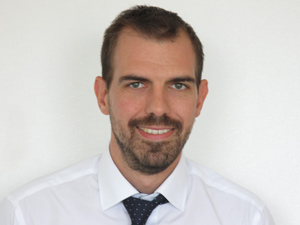
\includegraphics[width=0.25 \linewidth]{profil.png}	%trimming relative to image size!
\end{flushright}
\end{figure}

%---------------------------------------------------------------------------------------
%	QR CODE (optional)
%----------------------------------------------------------------------------------------
%\vspace{-136pt}
%\hspace{0.75\linewidth}
%\includegraphics[width=103pt]{qrcode}
%\normalsize
%\vspace{88pt}

%---------------------------------------------------------------------------------------
%	META SECTION
%----------------------------------------------------------------------------------------

\vspace{-114pt}

\metasection{Titre}{Consultant Senior pour Smartwave (8 ans) puis TALAN Suisse (depuis 8 mois), Permis G}
\metasection{Expertise}{Analyse et conduite de projets dans la transformation digitale} 
\metasection{Compétences}{Excellente maîtrise de Java et du Framework Spring.  Connaissances approfondies sur Angular, Git et Maven. Capable d'apprendre et maîtriser rapidement de nouvelles technologies}
\metasection{Hobbies}{Basket, Cinéma, Litérature, \OE{}nologie}

\vspace{6pt}

%---------------------------------------------------------------------------------------
%	SUMMARAY (optional)
%----------------------------------------------------------------------------------------

%\cvsection{Summary}\\
%Digital media graduate with four years project experience in the field of technology based assessment. Specialized in development of test-scenario engines and innovative, rich media item formats. Master studies focused on teams from different disciplines and cultural backgrounds on solutions for complex problems.  Prior knowledge has been collected in he field of usability / accessibility during bachelor studies.\\

%============================================================================%
%
%	CV SECTIONS AND EVENTS (MAIN CONTENT)
%
%============================================================================%

%---------------------------------------------------------------------------------------
%	EXPERIENCE
%----------------------------------------------------------------------------------------
\cvsection{Expérience}

\cveventc{2020}{Conges}{Pictet}{Visualisation et quittancement des activités journalières des comptes bancaires par les gérants}{Analyse technique, estimation, développement et automatisation des tests Back-end et Front-end}{Java 8, Spring Boot, Spring Sécurity, DDD, Cucumber, Angular 7, Maven, Git, OpenAPI, JIRA, Kubernetes, Sonar, Bamboo}

\cvevent{2019}{Entrée chez TALAN Suisse SA}{}

\cveventc{2019}{Framework pour solutions digitales Java}{UBP}{Architecte et tech leader des solutions digitales Java de la banque}{Création d'un Starter Spring Boot simplifiant la mise en place nouveau projets et respectant les règles d'implémentation et de sécurité imposées par la banque pour ses services digitaux. Environ une dizaine de projets impactés pour une équipe de 8 personnes}{Java 8, Spring Boot, Spring Sécurity, Kerberos, Maven, Swagger, JIRA}

\cveventc{2018}{Credit Protocols}{UBP}{Tech Leader d'un outil de simulation des crédits bancaires}{Intégration avec différentes solutions de la banque dont Appway, PrintNet et Documentum. Création de documents confidentiels destinés au Comité d'Administration}{Java 8, AngularJS, Spring Boot, Kerberos, Appway, PrintNet, Documentum, Maven, Swagger, JIRA}

\cveventc{2017}{Security Transfer Application}{UBP}{Analyse et développement d'un outil de traitement des transferts bancaires internationaux. Réalisation et estimations du projet. Intégrations avec le Core Banking. Création d'une interface configurable d'édition des SWIFT}{Le projet est utilisé par plus de 600 gérants dans le monde et permet de transférer environ 100 milliards de CHF/an}{Java 8, AngularJS, Spring Boot, Kerbeors, Documentum, SWIFT, Maven, IBM IQ, Swagger, JIRA}

\cveventb{2016}{Maintenance et support Documentum}{UBP}{Configuration d'interfaces D2. Création de TBO. Installation de Docbase. Digitalisation des services Documentum en REST via Spring Boot}{Java 8, Spring Boot, Kerberos, Documentum, Composer, Maven}

\pagebreak
\cvsection{Expérience (suite)}

\cveventc{2016}{Evolution de la visionneuse WEASIS}{HUG}{Projet Open Source en OSGI conçu et maintenu par le service d'imagerie médicale}{Création d'un module d'import d'images non radiologiques. Ajout d'outils de retouche et classement dans le Dossier Patient}{Java 8, Git, OSGI, Elasticsearch, Spring Boot, DICOM}

\cveventc{2015}{Leader Technique du projet UN Portal}{WTO}{Création d'un portail web microservices. L'application est destinée prioritairement aux membres des Organisations internationales, leur fournissant un moyen unique d'authentification}{ Le premier service implémenté fut destiné à l'enregistrement des délégations internationales pour les ministérielles de décembre 2015}{IntelliJ, JHipster, Java 7, AngularJS, Spring Boot, Docker, Git, Bower}


\cveventb{2014}{Webinar Bonita}{{\small Smartwave / Bonita Soft}}{Présentation d’un webinar sur l'utilisation l’outil Bonita Studio dans le cadre du développement d'applications mobiles}{IntelliJ, Java7, JHipster, Bonita Studio, IONIC, AngularJS}

\cveventb{2014}{Software Factory et industrialisation de Documentum}{{\small Phillip Morris International}}{Installation complète d'une Software Factory. Aide à la mise en place d'outils de contrôle qualité sur Documentum}{Maven, Junit, Jenkins, Sonar, Artifactory, Documentum}

\cveventb{2014}{Initiateur du projet Social Media}{Firmenich}{Réalisation d'un \emph{proof of concept} analysant en temps réel des mots clés sur Twitter. Les données collectées sont utilisées par le service Marketing afin d'anticiper de nouvelles tendances}{Elasticsearch, Kibana, AngularJS, AWS}

\cveventb{2013}{Développeur Flex}{Pictet}{Evolution des 2 projets Flex initiés en 2012. Gestion de l'impression PDF}{Java,  JUnit, Hibernate, Oracle, Git, Dozer mapping, Flex, JIRA}

\cveventb{2012-2013}{Développeur JBoss Seam}{EBU-UER}{Conception et développement d'un Purchase Order System en JBoss Seam. Développement de composants, responsable du design Front-End, création d'un outil d'aide à l'estimation des coûts configurable}{Eclipse, JEE6, Jboss Seam 3, JPA, JSF2, Bootstrap, JQuery, WSO2 ESB}

\cveventb{2012}{Développeur Flex}{Pictet}{Développement à partir d'un projet existant d'une seconde version. Mutualisation de composants Front-End et Back-End}{FlexBuilder, Hibernate, Flex, Maven, JIRA}

\cveventb{2010-2012}{Consultant Java/JBoss Seam}{Merck Serono}{Estimation, conception et maintenance d'application web  JBoss Seam}{Eclipse, JBoss/Seam, Hibernate, JQuery, Oracle 10g, SVN, Drools}

\cvevent{2011}{Entrée chez Smartwave}{}

\pagebreak
\cvsection{Expérience (suite)}

\cveventb{2010-2011}{Responsable de l'application Igor}{{\small Orange Business Services}}{Suivi des évolutions d'un ETL développé par les équipes d'Atos Origin}{Eclipse, Oracle, SVN, SQL, XML, HPQC, Ant}

\cveventb{2009}{Projet de refonte Tolologique}{{\small Orange Business Services}}{Refonte d'un projet veillissant en Flex 4. Responsable de l'intégration Client-Server. Création d’un outil de transformation des fichiers SVG en FXG via un script XSLT}{Eclipse, Flex 4, CVS, XSLT, JAVA/J2EE, JavaScript}

\cveventb{2008-2011}{Responsable de l'application TCSNMP}{{\small Orange Business Services}}{Ecriture des spécifications de demandes d'évolutions et estimations. Mise à jour des règles d’identification JRules. Amélioration permanente de la qualité via Hudson et Sonar.}{Linux(Platon), Eclipse, JRules, SVN, Java/JUnit, Maven, Hudson, Sonar}

\cvevent{2008}{Entrée chez Atos Origin}{}

\bigskip 

%---------------------------------------------------------------------------------------
%	EDUCATION SECTION
%--------------------------------------------------------------------------------------
\cvsection{Formations et certifications}

\cvevent{2017}{Accrédité SECRET par l'UBP}{Suisse}

\cvevent{2017}{Formation \textit{Architecting Documentum Applications}}{Suisse}

\cvevent{2015}{Formation \textit{Excellence dans la relation clientèle}}{Suisse}

\cvevent{2014}{Certifié SAP Fiori UX}{Suisse}

\cvevent{2012}{Certifié WSO2 ESB developer}{Londres}

\bigskip

\cvsection{Parcours Académique}

\cvevent{2008}{Master 2 - Informatique (Mention Bien)}{Université du Havre}

\cvevent{2007}{Master 1 - Informatique (Mention Assez Bien)}{Université du Havre}

\cveventb{2006}{Dundalk Institute of Technologie}{Irlande}{Bachelor of science in computing in software development (with merit)}{DUETI - Diplôme Universitaire d'Etudes Technologiques Internationales}

\cveventa{2003 - 2005}{DUT Informatique}{IUT du Havre}{Option Génie Logiciel}

\cveventa{Juin 2003}{Bac Scientifique}{Le Havre}{Spécialité Mathématiques}
%\textcolor{softcol}{\hrule}

%-------------------------------------------------------------------------------------------------
%	ARTIFICIAL FOOTER (fancy footer cannot exceed linewidth) 
%--------------------------------------------------------------------------------------------------

\null
\vspace*{\fill}
\hspace{-0.25\linewidth}\colorbox{bgcol}{\makebox[1.5\linewidth][c]{\mystrut \small \textcolor{white}{larvor.yannick@gmail.com} $\cdot$ \textcolor{white}{github.com/ratonlarvor}}}




%============================================================================%
%
%
%
%	DOCUMENT END
%
%
%
%============================================================================%
\end{document}
